\documentclass[14pt,mathserif]{beamer}
\usepackage[noend]{algorithmic}
\usepackage{latexsym,amsmath,url}
\usepackage{hyperref}
\DeclareSymbolFont{AMSb}{U}{msb}{m}{n}
\DeclareMathSymbol{\N}{\mathbin}{AMSb}{"4E}
 \DeclareMathOperator*{\argmax}{argmax}
 \DeclareMathOperator*{\sign}{sign}
\newcommand{\vecb}[1]{\mathbf{#1}}
\newcommand{\x}{\mathbf{x}} 
\newcommand{\y}{\mathbf{y}}
\newcommand{\w}{\mathbf{w}}

\newcommand{\superscript}[1]{\ensuremath{^\textrm{\scriptsize#1 }}}
\mode<presentation>{ 
  \usetheme{Boadilla}
} \title[ML / NLP / MT Course ]{ Machine Learning for NLP and MT }


\author[Chrupala and Stroppa]{Grzegorz Chrupa{\l}a and Nicolas Stroppa}

\institute[Saarland+Google] % (optional, but mostly needed)
{
Saarland University\\
Google
}
\date[2010] % (optional, should be abbreviation of conference name)
{META Workshop}


%\pgfdeclareimage[height=1cm]{UdS}{SaarlandUniversityLogo.jpg}
%\logo{\pgfuseimage{UdS}}

 \AtBeginSection[]
 {
    \begin{frame}
        \frametitle{Outline}
        \tableofcontents[currentsection]
    \end{frame}
 }
\begin{document}
\frame{\titlepage}

\begin{frame}
  \frametitle{Outline}
  \tableofcontents
\end{frame}

\section{Linear models}

\begin{frame}
  \frametitle{Linear models}
  \begin{block}{}
    Think of training examples as points in $d$-dimensional
    space. Each dimension corresponds to one feature.
  \end{block}
  \begin{block}{}
    A linear binary classifier defines a plane in the space which
    separates positive from negative examples. 
  \end{block}

\end{frame}

\begin{frame}
 \frametitle{Linear decision boundary}
\begin{itemize}
\item A \alert{hyperplane} is a generalization of a straight line to
  $>2$ dimensions
\item A hyperplane contains all the points in a $d$ dimensional space satisfying the following equation:
\[
 w_1x_1 + w_2x_2, \ldots, + w_dx_d + w_0 = 0
\]
\item Each coefficient $w_i$ can be thought of as a weight on the
  corresponding feature
\item The vector containing all the weights $\w = (w_0,\ldots,w_d)$ is the
  \alert{parameter vector} or \alert{weigth vector}
\end{itemize}
\end{frame}



\begin{frame}
 \frametitle{Normal vector}
\begin{itemize}
\item Geometrically, the weight vector $\w$ is a \alert{normal vector}
  of the separating hyperplane
\item A normal vector of a surface is any vector which is
  perpendicular to it
\begin{center}
 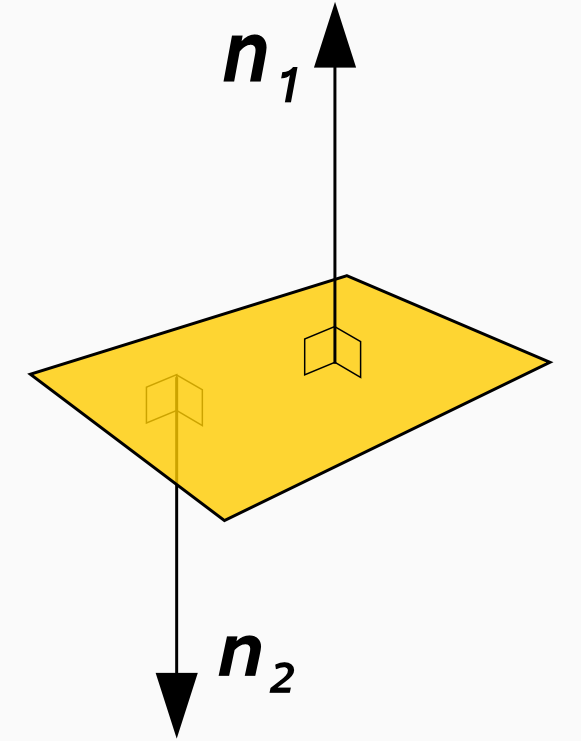
\includegraphics[scale=0.2]{Normal_vectors2.png}
 \end{center}
\end{itemize}
\end{frame}


 \begin{frame}\frametitle{Hyperplane as a classifier}
   \begin{itemize}
   \item Let \[
     g(\x) =  w_1x_1 + w_2x_2, \ldots, + w_dx_d + w_0
     \]
 \item Then
   \[ y = 
   \begin{cases}
    +1 & \text{ if } g(\x) \geq 0\\
    -1 & \text{ otherwise }
   \end{cases}
 \]
   \end{itemize}
 \end{frame}

\begin{frame}
 \frametitle{Bias}
\begin{itemize}
\item The slope of the hyperplane is determined by
  $w_1...w_d$. The location (intercept) is determined by  bias $w_0$
\item Include bias in the
  weight vector and add a dummy component to the feature vector
\item Set this component to $x_0 = 1$
\item Then 
 \begin{align}
 g(\x) & = \sum_{\alert{i=0}}^d w_i x_i\\
 g(\x) & = \w \cdot \x
\end{align}
\end{itemize}
\end{frame}

\begin{frame}
\label{hyperplanes}
 \begin{center}\frametitle{Separating hyperplanes in 2 dimensions}
\vskip -0.5cm 
\includegraphics[scale=0.5]{linear.pdf}
\end{center}
\end{frame}



\section{Perceptron}
\begin{frame}
 \frametitle{Perceptron training}
\begin{itemize}
 \item How do we find a set of weights that separate our classes?
\item \textbf{Perceptron}: A simple mistake-driven online algortihm
\begin{block}{}
\begin{itemize}
\item Start with a zero weight vector and process each training
  example in turn.
\item If the current weight vector classifies the current example
  incorrectly, move the weight vector in the right direction.
\item If weights stop changing, stop
\end{itemize}
\end{block}
\item If examples are linearly separable, then this algorithm is
  guaranteed to converge to the solution vector
\end{itemize}
\end{frame}

\begin{frame}
 \frametitle{Fixed increment online perceptron algorithm}
\begin{itemize}
\item Binary classification, with classes $+1$ and $-1$
\item Decision function $y' = \mathrm{sign}(\vecb{w}\cdot \x)$
\end{itemize}

\begin{block}{\textsc{Perceptron}($x^{1:N},y^{1:N},I$):}
\begin{algorithmic}[1]
\STATE $\vecb{w} \leftarrow \vecb{0}$
\FOR {$i = 1...I$}
	\FOR {$n = 1...N$}
    		\IF {$y^{(n)} (\vecb{w}\cdot \x^{(n)}) \leq 0$}
        		\STATE $\vecb{w} \leftarrow \vecb{w} + y^{(n)} \x^{(n)}$
    		\ENDIF
    	\ENDFOR
\ENDFOR
\STATE \textbf{return} $\vecb{w}$
\end{algorithmic}                 \end{block}
\end{frame}


\begin{frame}
  \frametitle{Or more explicitly}
\begin{algorithmic}[1]
\STATE $\vecb{w} \leftarrow \vecb{0}$
\FOR {$i = 1...I$}
  \FOR {$n = 1...N$}
    \IF {$y^{(n)} = \sign(\w\cdot \x^{(n)}) $}
      \STATE pass
      \ELSIF { $y^{(n)} = +1 \wedge \sign(\w\cdot\x^{(n)}) = -1$ }
      \STATE $\w \leftarrow \w + \x^{(n)}$
      \ELSIF { $y^{(n)} = -1 \wedge \sign(\w\cdot\x^{(n)}) = +1$ }
      \STATE $\w \leftarrow \w - \x^{(n)}$
    \ENDIF
   \ENDFOR
  \ENDFOR
\STATE \textbf{return} $\vecb{w}$
\end{algorithmic}
\end{frame}

\begin{frame}
 \frametitle{Weight averaging}
\begin{itemize}
\item Although the algorithm is guaranteed to converge, the solution
  is not unique!
\item Sensitive to the order in which examples are processed
\item Separating the training sample does not equal good accuracy on
  unseen data
\item Empirically, better generalization performance with
  \alert{weight averaging}
\begin{itemize}
\item A method of avoiding overfitting
\item As final weight vector, use the mean of all the weight vector
  values for each step of the algorithm
\end{itemize}
\end{itemize}
\end{frame}


\section{Na{\"i}ve Bayes}
\begin{frame}
  \frametitle{Probabilistic model}
  \begin{itemize}
  \item Instead of thinking in terms of multidimensional space...
  \item Classification can be approached as a probability estimation problem
  \item We will try to find a probability distribution which
    \begin{itemize}
    \item  Describes
    well our training data 
  \item Allows us  to make accurate predictions 
    \end{itemize}
  \item We'll look at Naive Bayes as a simplest example of a
    probabilistic classifier
  \end{itemize}
\end{frame}

\begin{frame}
  \frametitle{Classes and features as random variables}
  \begin{itemize}
  \item Let $Y$ be a random variable ranging over our classes. 
  \item For binary classification $Y=+1$ or $Y=-1$
  \item Let $X_1 ... X_d$ be random variables corresponding to
    features. 
  \item For a document, we could have:

    \begin{tabular}{rlllll}
          &    $X_1$& $X_2$   & $X_3$   & $X_4$   & \\\hline
          & Obama   & Ferrari & voters  & movies & \\\hline
$x = ($   & 1       & 0       & 1       & 0 & $)$\\
    \end{tabular}
  \end{itemize}
\end{frame}

\begin{frame}
  \frametitle{Probability}
  \begin{block}{}
We need to estimate 
\[
P(Y=+1|X=x) = P(Y=+1|X_1=x_1\ldots X_d=x_d) 
\]
\end{block}
\begin{itemize}
\item But conditioning on $X$ is very hard due to sparseness,
  especially for high dimensional data.
\item So, let's use Bayes rule.
\end{itemize}
\end{frame}

\begin{frame}
  \frametitle{Bayes rule} Bayes rule determines how joint and
  conditional probabilities are related.
 
  \begin{block}{}
\[
    P(Y=y_i|X=x) = \frac{P(X=x|Y) P(Y=y_i)}{\sum_i P(X=x|Y=y_i)
      P(Y=y_i)}
\]
That is:
\[
\mbox{posterior} = \frac{\mbox{prior} \times \mbox{likelihood}}{\mbox{evidence}}
\]
\end{block}
\end{frame}

\section{Logistic regression}

\section{Extra material}
\begin{frame}
\frametitle{Efficient averaged perceptron algorithm}
 \begin{block}{\textsc{Perceptron}($x^{1:N},y^{1:N},I$):}
\begin{algorithmic}[1]
\STATE $\vecb{w} \leftarrow \vecb{0}$ ; $\vecb{w_a} \leftarrow \vecb{0}$
\STATE $b \leftarrow 0$ ; $b_a \leftarrow 0$
\STATE $c \leftarrow 1$
\FOR {$i = 1...I$}
	\FOR {$n = 1...N$}
    		\IF {$y^{(n)} (\vecb{w}\cdot \x^{(n)}+b) \leq 0$}
        		\STATE $\vecb{w} \leftarrow \vecb{w} + y^{(n)} \x^{(n)}$ ; $b \leftarrow b + y^{(n)}$
			\STATE $\vecb{w_a} \leftarrow \vecb{w_a} + c y^{(n)} \x^{(n)}$ ; $b_a \leftarrow b_a + c y^{(n)}$

    		\ENDIF
        \STATE $c \leftarrow c + 1$
    	\ENDFOR
\ENDFOR
\STATE \textbf{return} $(\vecb{w}-\vecb{w_a}/c, b - b_a/c)$
\end{algorithmic}                 \end{block}
\end{frame}


\end{document}
